\documentclass[titlepage]{article}
\usepackage{algpseudocode}
\usepackage{algorithm}
\usepackage{graphicx} % Required for inserting images
\usepackage[utf8]{inputenc}
\usepackage{setspace}
\usepackage{amssymb}
\usepackage{amsmath}
\usepackage{listings}
\usepackage{matlab-prettifier}
\usepackage{url}
\usepackage{hyperref}
\usepackage{float}
\usepackage{caption}
\usepackage{subcaption}
\graphicspath{ {./Images/} }

\title{Sledenje žarku v neevklidskih prostorih}
\author{Blaž Bergant, Martin Jereb, Matjaž Pogačnik}
\date{Matematično modeliranje, maj 2024}

\begin{document}

\maketitle
\newpage
\tableofcontents
\newpage

\section{Uvod}
Algoritem sledenja žarku (\textit{ang. Ray Tracing}) je priljubljen algoritem, uporabljen v računalniški grafiki, ki simulira realistično osvetlitev prizorov. Temelji na ideji sledenja žarka svetlobe po prizoru, izračunavanju njegovega preseka z objekti in odbijanju v drugo smer. Običajno ta algoritem uporabljamo v običajnem evklidskem prostoru, saj predstavlja resnični svet. Vendar pa lahko algoritem implementiramo tudi v drugih (neevklidskih) prostorih, da dobimo zanimive vizualne rezultate. To bo glavna naloga tega projekta.

\section{Cilji}
Cilji za to projektno nalogo so implementacija "osnovnega" algoritma sledenje žarkom v evklidskem prostoru, njegova nadgradnja, da deluje tudi v neevklidskem prostoru na ploščatem torusu in 2-sferi ter primerjava delovanja v evklidskem in neevklidskem prostoru.

\section{Sledenje žarkom}
Predstavljajmo si, da smo na plaži v naši najljubši obalni turistični destinaciji in gledamo, kako bližnja barka pluje v sončni zahod. Nam, na obali, zgleda, da se poleg oddaljevanja tudi "pogreza" v tla. Zakaj pa je temu tako? 

To je ravno zaradi potovanja žarkov. Ker smo v evklidskem prostoru, bo žarek potoval naravnost in nas zaradi ukrivljenosti Zemlje tako, po določeni razdalji, ne bo več dosegel. Sedaj, pa si predstavljajmo, da bi lahko barko kljub oddaljevanju še vedno videli celotno. Ta posebna zmožnost, bi nam bila omogočena v neevklidskem prostoru. In sicer še bolj natančno, v sferičnem neevklidskem prostoru.

\begin{figure}[H]
    \centering
    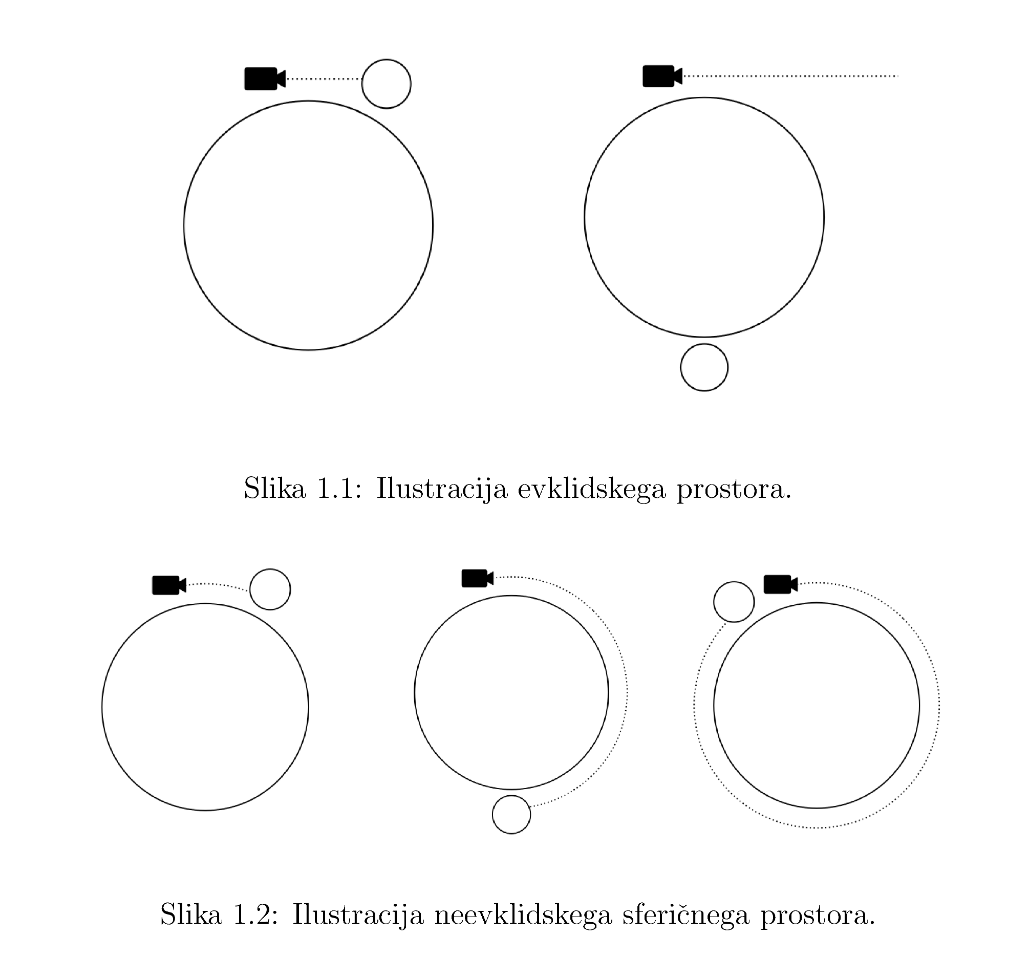
\includegraphics[width=0.5\linewidth]{Images/potovanje_zarkov.png}
    \caption{Primerjava [Vir: G. Kovač]}
    \label{Slika:Primerjava}
\end{figure}

Kaj pa pravzaprav je neevklidski prostor?
Neevklidski prostor je preprosto prostor, ki ne sledi pravilom evklidske geometrije. Torej prostor ni raven ampak je ukrivljen, vsota kotov v trikotniku je večja ali pa manjša od 180 stopinj... Neevklidski prostor delimo na več različnih geometrij med katerimi so recimo hiperbolična geometrija, eliptična geometrija, sferična geometrija, projektivna geometrija...

\section{Implementacija osnovnega algoritma ray tracing}
Vsak objekt v prostoru opisuje enačba oblike:
\begin{equation}
    f(x,y,z)=0
\end{equation}

Naš program je sposoben upodobiti preprost prizor z osnovnim senčenjem po naslednjem postopku:
\newline
\bigskip
\begin{enumerate}
  \item 
\item V poljubnem prostoru premikamo žarek za nek korak, kjer vsakič preverimo, če se je $f$ v novi točki spremenil predznak.
\item Poiščemo natančnejše presečišče tako, da razpolavljamo korak, doker se uspešno ne premaknemo naprej brez spremembe predznaka. Naprej se spet premikamo, doker se ne spremeni predznak. Postopek ponavljamo, doker nismo od objekta oddaljeni za manj kot $\varepsilon$.
\begin{figure}[H]
    \centering
    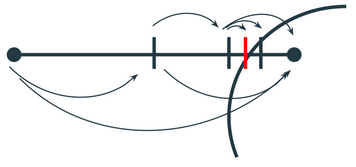
\includegraphics[width=0.5\linewidth]{intersect.png}
    \caption{Iskanje natančnejšega presečišča}
    \label{Slika:Iskanje natančnejšega presečišča}
\end{figure}
\item[] V našem prostoru so bili objekti dveh tipov. Sfere s središčem v $(x_{0}, y_{0}, z_{0})$ in polmerom $r$, podane v obliki $(x-x_{0})^{2}+(y-y_{0})^{2}+(z-z_{0})^{2}=r^{2}$ in ravnine podane z $ax+by+cz=d$. Razdalja točke do sfere je bila izračunana kot
\begin{equation} \label{e:distSphere}
    l=\left \| \vec{r}_{t}-\vec{r}_{ci} \right \| - r
\end{equation}
kjer je $\vec{r}_{t}$ krajevni vektor točke žarka, $\vec{r}_{ci}$ pa krajevni vektor središča sfere, razdalja do ravnine pa kot
\begin{equation} \label{e:distPlane}
    l=\frac{\left | ax_{t}+by_{t}+cz_{t}-d \right |}{\sqrt{a^{2}+b^{2}+c^{2}}}
\end{equation}
kjer so $x_{t}, y_{t}, z_{t}$ koordinate točke žarka.
\item Žarek nato pošljemo od presečišča v smeri proti viru svetlobe, pri tem pa preverjamo presečišča podobno kot pri (1.)
\end{enumerate}
Vsak žarek predstavlja piksel na končni sliki. Če se je žarek sekal s katerim od objektov, mu pripišemo barvo tega objekta. Če žarek v nadaljevanju ni uspešno prišel do vira svetlobe, barvo prvotnega žarka nekoliko zatemnimo (RGB vrednosti pomnožimo z nekim faktorjem $\alpha < 0$)

\bigskip
V nadaljevanju smo implementirali algoritem za sledenje žarku na tridimenzionalnem ploščatem torusu $\mathbb{T}_{pl}^{3}$ in dvodimenzionalni sferi $\mathbb{S}^2$ v $\mathbb{R}^3$. Algoritem za sledenje žarku v evklidskem prostoru je enak algoritmu za torus, brez preslikave žarka na željeno domeno. Sledenje v smeri vira svetlobe uporablja algoritem za sledenje žarku v evklidskem prostoru, pri tem pa ga pri korakih dolžine $h$ omejimo na maksimalno število korakov
$k_{max}= \left \lceil \frac{\left \|\vec{r}_{l}-\vec{r}_{t} \right \|}{h} \right \rceil$, kjer je $\vec_{r}_{l}$ krajevni vektor vira svetlobe,
$\vec_{r}_{t}$ pa krajevni vektor točke presečišča.

\section{Sledenje žarkom na ploščatem torusu $\mathbb{T}_{pl}^{3}$} 
\subsection{Kaj je tri dimenzionalni ploščati torus?}
Tri dimenzionalni ploščati torus \( \mathbb{T}^3_{pl} \), je tridimenzionalna mnogoterost v evklidski geometriji. \( \mathbb{T}^3_{pl} \) dobimo tako, da "zlepimo" nasprotne ploskve enotske kocke \([0,1] \times [0,1] \times [0,1] \subset \mathbb{R}^3 \), kjer je \(\mathbb{R}^3\) tridimenzionalni evklidski prostor. Formalno pravimo, da je \( \mathbb{T}^3_{pl} \) kvocient \(\mathbb{R}^3\) z grupo translacij:
\[
(x, y, z) \to (x \pm 1, y, z), \quad (x, y, z) \to (x, y \pm 1, z), \quad (x, y, z) \to (x, y, z \pm 1).
\]

Običajni torusi so ukrivljeni in se jim ukrivljenost po površini spreminja. Ploščati torus pa ima konstantno ukrivljenost v vsaki točki. Poimenovanje ploščat izhaja iz tega, ker je povsod podoben navadni evklidski ravnini. Podobno velja za tridimenzionalni ploščati torus, kjer pri sledenju žarka lahko uporabimo kar osnovno definicijo žarka. Ključna razlika med algoritmom v \( \mathbb{R}^3 \) in \( \mathbb{T}^3_{pl} \) pa je, da bomo tokrat dodali še en korak, ker moramo žarek omejiti na enotsko kocko. Dokler se nahajamo znotraj njenih meja, ne naredimo nobenih popravkov. Ko pa ugotovimo presečišče z eno od ploskev, moramo žarek preslikati na nasprotno ploskev. To lahko storimo tako, da preprosto od žarka odštejemo normalo ploskve, na kateri smo.

\begin{figure}[H]
    \centering
    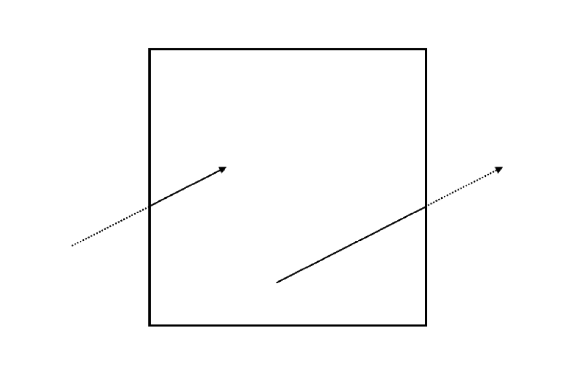
\includegraphics[width=0.5\linewidth]{Images/flat_torus_zrcaljenje.png}
    \caption{Žarek v dvodimenzionalnem ploščatem torusu}
    \label{Slika:Žarek v dvodimenzionalnem ploščatem torusu}
\end{figure}

\subsection{Razlaga kode}
Ključni vpogled, je da žarek omejimo, kar lahko v programskih jezikih storimo preprosto z operatorjem modulo. Rešitev torej dobimo, ko žarek preslikamo z modulo 1 in tako rezultat omejimo na enotsko kocko.
        
\begin{align*}
x &= \left( \text{x} + \text{korak} \cdot \text{smer x} \right) \mod 1 \\
y &= \left( \text{y} + \text{korak} \cdot \text{smer y} \right) \mod 1 \\
z &= \left( \text{z} + \text{korak} \cdot \text{smer z} \right) \mod 1
\end{align*}

% added
% TODO: formule za mapiranje žarka na zeljeno domeno

Funkciji \textbf{signs} in \textbf{checkIntersect} implementirata funkcije $f$, \textbf{distance} pa implementira formuli \eqref{e:distSphere} in 
\eqref{e:distPlane}. Funkcija \textbf{remap} implementira formule %TODO: link enacbe
\begin{algorithm}
    \caption{Sledenje žarku na ploščatem torusu}
\begin{algorithmic}
    \Function{traceRayFlatTorus}{$T_{0}$, $\vec{v}$, step, maxIt, objects, a, b, $\varepsilon$}

    \State $T_{n}$, $T_{n+1}$ $\gets$ $T_{0}$
    \State signs $\gets$ \textbf{signs}($T_{n}$, objects)
    \Comment{izračunamo začetne predznake}
    \\
  \While{true}
    \If{step == maxIt}
      \State \Return{-1}
    \ElsIf{\textbf{distance}($T_{n}$, objects) $<$ $\varepsilon$}
      \State \Return{$T_{n}$}
    \EndIf
    \State $T_{n+1}$ $\gets$ $T_{n}+step \cdot \vec{v}$
    \State $T_{n+1}$ $\gets$ \textbf{remap}($T_{n+1}$, a, b)
    \\
    \Comment{naredimo korak, preslikamo na željeno domeno}
    \\
    \State signs $\gets$ \textbf{checkIntersects}($T_{n+1}$, objects, signs)
    \\
    \Comment{preverimo, če smo sekali objekt}
    \\
    \Comment{če da, razpolovimo korak}

    \If{object != NULL}
        \State step $\gets$ step/2
    \Else
      \State $T_{n}$ $\gets$ $T_{n+1}$
    \EndIf
  \EndWhile
\EndFunction
\end{algorithmic}
\end{algorithm}

% ----

Ko program poženemo, dobimo lep vizualni rezultat.
\begin{figure}[H]
    \centering
    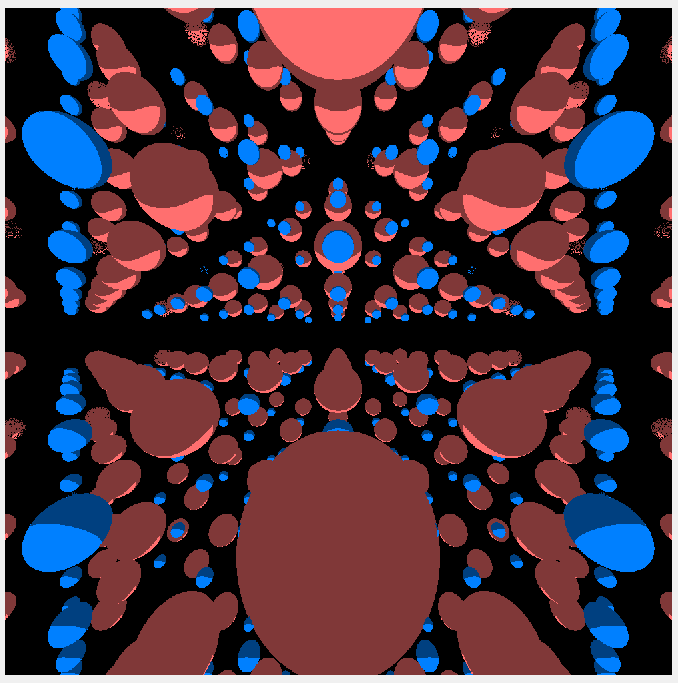
\includegraphics[width=0.5\linewidth]{Images/flat_torus.png}
    \caption{Rezultat "ray tracinga" za tri dimenzionalni ploščati torus}
    \label{Slika:Rezultat "ray tracinga" za tri dimenzionalni ploščati torus}
\end{figure}
Na sliki lahko opazimo, da so elementi simetrično preslikani, prav tako pa lahko vidimo, da so tudi različno osenčeni.

\section{Sledenje žarkom na dvodimenzionalni sferi $\mathbb{S}^{2}$}
Žarek na dvodimenzionalni sferi bo potoval po najravnejši poti, tj. geodetki. Geodetka je krivulja po sferi, kjer zahtevamo, da je
pospešek v smeri normale tangentne ravnine 0. Majhen korak po geodetki je v $uv$ ravnini opisan s sistemom dveh diferencialnih enačb drugega reda.
\begin{equation}
    \begin{split}
        &\frac{d^{2}u}{dt^{2}}-\cos(u)\sin(u)\frac{dv}{dt}\frac{dv}{dt}=0 \\
        &\frac{d^{2}v}{dt^{2}}+2\cot(u)\frac{du}{dt}\frac{dv}{dt}=0
    \end{split}
\end{equation}

Po krivulji se bomo v nadaljnjih algorimih premikali s pomočjo aproksimacijskih metod, zato moramo sistem DE drugega reda preoblikovati v
sistem DE prvega reda. Za to uvedemo 4 nove spremenljivke
\begin{equation}
\begin{split}
    &y_{1}=u, \quad y_{2}=\frac{dy_{1}}{dt}, \\
    &y_{3}=v, \quad y_{4}=\frac{dy_{3}}{dt}
\end{split}
\end{equation}
Dobimo sistem 4 DE prvega reda
\begin{equation} \label{e:geoSys}
\begin{split}
    &\frac{dy_{1}}{dt}=y_{2} \\
    &\frac{dy_{2}}{dt}=\cos(y_{1})\sin(y_{1})y^{2}_{4} \\
    &\frac{dy_{3}}{dt}=y_{4} \\
    &\frac{dy_{4}}{dt}=-2\cot(y_{1})y_{2}y_{4}
\end{split}
\end{equation}
Ker se bomo premikali po $uv$ ravnini, moramo koordinate v kartezičnem koordinatnem sistemu transformirati v parametra $u$ in $v$. Sfera v $\mathbb{R}^3$ je
parametrizirana kot
\begin{equation} \label{e:toXYZ}
    \begin{split}
        &X=R\cos(v)\sin(u) \\
        &Y=R\sin(v)\sin(u) \\
        &Z=R\cos(u)
    \end{split}
\end{equation}
$u$ lahko dobimo kot
\begin{equation}
        u=\cos^{-1} \left( \frac{X}{R} \right)
\end{equation}
za $v$ pa uporabimo prvi dve enačbi
\begin{equation} \label{e:toU}
    \begin{split}
        &\frac{R\sin(u)Y}{R\sin(u)X}=\frac{\sin(v)}{\cos(v)} \\
        &v=\tan^{-1} \left(\frac{Y}{X} \right)
    \end{split}
\end{equation}

Za sledenje žarku po geodetki, si moramo poleg začetne točke izbrati še začetno smer
$\left( \frac{du}{dt}, \frac{dv}{dt} \right)$. Tako kot pri ostalih prostorih v nalogi, bomo uporabili "FOV" način
potovanja žarkov iz kamere. Od tu dalje imamo svobodo pri izbiri sfer, po katerih bodo žarki potovali. V tej nalogi smo za
vsak žarek izračunali središče sfere z najnižjo $z$ koordinato in polmerom $R$, žarki pa bodo vedno "zavijali" navzdol, torej se bodo premikali po poldnevnikih.

\begin{figure}[H]
\centering
\begin{minipage}{.5\textwidth}
  \centering
  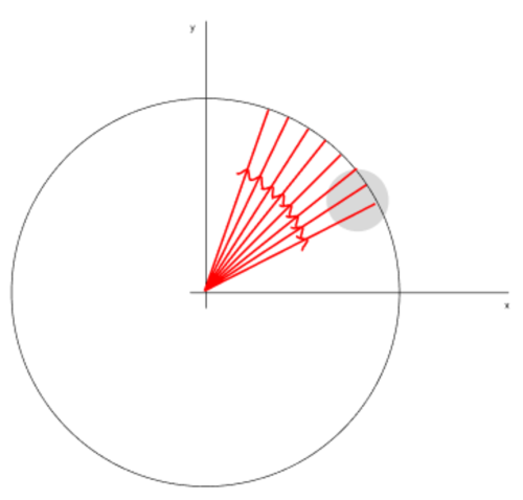
\includegraphics[width=0.8\linewidth]{Images/rays_top.png}
  \captionof{figure}{Potovanje žarkov od zgoraj}
  \label{fig:test1}
\end{minipage}%
\begin{minipage}{.5\textwidth}
  \centering
  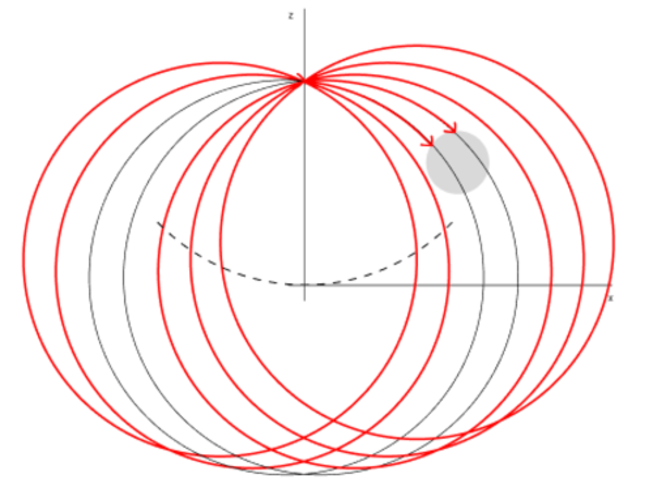
\includegraphics[height=0.77\linewidth]{Images/rays_side.png}
  \captionof{figure}{Potovanje žarkov s strani}
  \label{fig:test2}
\end{minipage}
\end{figure}

Središča sfer žarkov se bodo torej nahajala na sferi s polmerom $R$ in središem v kameri $T_{0}$. Za različne smeri žarkov $\vec{v}_{i}$ je bilo središče $C_{i}$ izračunano po sledečem postopku

\bigskip

Izračunamo vektorski produkt med navpičnim vektorjem in smerjo $\vec{v}_{i}$. Dobljeni vektor je normala na ravnino krožnice z iskanim središčem, ki gre skozi $T_{0}$
\begin{equation} \label{e:sphC1}
    \vec{n}_{i}=(0, 0, -1) \times \vec{v}_{i}
\end{equation}
Vektor, ki od $T_{0}$ kaže proti iskanemu središču bo ležal v tej ravnini, poleg tega pa bo pravokoten na $\vec{v}_{i}$. Ponovno uporabimo vektorski
produkt
\begin{equation}\label{e:sphC2}
    \vec{c}_{i}= \vec{v}_{i} \times \vec{n}_{i}
\end{equation}
Krajevni vektor središča nato dobimo tako, da se premaknemo za polmer $R$ v smeri $\vec{c}_{i}$
\begin{equation}\label{e:sphC3}
    \vec{r}_{ci}=\frac{\vec{c}_{i}}{\left \| \vec{c}_{i}\right \|} \cdot R + T_{0}
\end{equation}

Za korak po geodetki bomo $T_{0}$ najprej premaknili za vektor $\vec{r}_{ci}$, tako da bo središče sfere v koordinatnem izhodišču. Nato naredimo
korak, novo točko $T_{i1}$ pa premaknemo nazaj za vektor $\vec{r}_{ci}$.
Ker želimo potovati po poldnevnikih, bomo za začetno smer $\left( \frac{du}{dt}, \frac{dv}{dt} \right)$ izbrali $\left( \pm1, 0 \right)$. Korak po poldnevniku bo v $xy$ ravnini tako že pravnilno obrnjen, določiti pa moramo predznak premika po $u$ glede na to, ali se premikamo v pravo smer $\vec{v}_{i}$. To preverimo s skalarnim produktom
\bigskip
\newline
Naredimo korak v smeri $\left( 1, 0 \right)$ in označimo dobljeno točko s $T_{t}$. Vektor v smeri od $T_{0}$ do $T_{t}$ označimo z $\vec{v}_{t}$.
Izračunamo skalarni produkt
\begin{equation} \label{e:dirCorr}
    a= \vec{v}_{i} \vec{v}_{t}^T
\end{equation}
Če se premikamo v pravi smeri, bo $a > 0$, drugače moramo za začetno smer izbrati negativni predznak.
\bigskip
\newline
V nadaljevanju se premikamo po geodetki z eno izmed aproksimacijskih metod. V splošnem lahko za take sisteme uporabimo Eulerjevo metodo
\begin{equation} \label{e:euler}
    \begin{split}
        &t_{n+1}=t_{n}+h \\
        &\vec{y}_{n+1}=\vec{y}_{n}+h \cdot \vec{f}(t_{n}, \vec{y}_{n})
    \end{split}
\end{equation},
problem pa se pojavi pri $\cot(y_{1})$ v eni izmed enačb, ki ima pole pri
$k\pi$, $k \in \mathbb{Z}$. Da se temu izognemo ne smemo uporabljati fiksne dolžine koraka, temveč moramo uporabiti adaptivne metode, kot je DOPRI5,
ki z uporabo večih metod estimira napako približka, in temu primerno prilagodi korak.
\bigskip
\newline
Algoritmi, ki implementirajo opisane metode so predstavljeni v naslednjem poglavju.
\newpage

\section{Algorimi za 2-sphere}
Funkcija \textbf{sphereCenter} implementira formule \eqref{e:sphC1}, \eqref{e:sphC2}, \eqref{e:sphC3}, \textbf{initializeSphere} formule \eqref{e:geoSys}, \eqref{e:toU}, \eqref{e:toV}, \eqref{e:dirCorr}, \eqref{e:euler}, \textbf{uvToVec} pa formulo \eqref{e:toXYZ}. Funkcija \textbf{DOPRI5} predstavlja implementacijo DOPRI5, ki naredi po en korak glede na trenutno velikost koraka, in skupaj s približkom vrne tudi novo velikost koraka. Tu lahko uporabimo tudi katero drugo adaptivno funkcijo. Ostale funkcije so opisane v
razdelku %TODO: link razdelek
\begin{algorithm}
    \caption{Sledenje žarku na sferi $\mathbb{S}^{2}$}
\begin{algorithmic}
    \Function{traceRayNonEuclidean}{$T_{0}$, $\vec{v}$, step, maxIt, objects, R, $\varepsilon$}

    \State $T_{n}$, $T_{n+1}$ $\gets$ $T_{0}$
    \State signs $\gets$ \textbf{signs}($T_{n}$, objects)
    \Comment{izračunamo začetne predznake}
    \State center, I
    \\
  \While{true}
    \If{step == maxIt}
    \State \Return{-1}
    \ElsIf{step == 0}
      \State center $\gets$ \textbf{sphereCenter}($T_{0}$, d, R)
      \\
      \Comment{žarku poiščemo središče sfere}
      \State $T_{m}$ $\gets$ $T_{0} - \hbox{center}$
      \Comment{sfero premaknemo v $(0, 0)$}
      \State $\vec{y}_{n}$ $\gets$ \textbf{initializeSphere}($T_{0}$, R)
      \Comment{pripravimo začetni $\vec{y}$}
    \EndIf
    \\
    \State $\vec{y}_{n+1}, \hbox{step}$ $\gets$ \textbf{DOPRI5}($\vec{y}_{n}$, step)
    \Comment{korak po geodetki}
    \State $T_{n+1}$ $\gets$ \textbf{uvToVec}($\vec{y}_{n+1}$, R) + center
    \\
    \State object $\gets$ \textbf{checkIntersects}($T_{n+1}$, objects, signs)
    \\
    \Comment{preverimo, če smo sekali objekt}
    \\
    \Comment{če da, poiščemo natančno presečišče}

    \If{object != NULL}
      \State I $\gets$ \textbf{findIntersection}($T_{n}$, object, signs, $\vec{y}_{n}$, step, R, center, $\varepsilon$)
      \State \Return{I}
    \Else
      \State $\vec{y}_{n}$ $\gets$ $\vec{y}_{n+1}$
      \State $T_{n}$ $\gets$ $T_{n+1}$
    \EndIf
  \EndWhile
\EndFunction
\end{algorithmic}
\end{algorithm}

\begin{algorithm}[H]
    \caption{Iskanje natančnejšega presečišča}
\begin{algorithmic}
    \Function{findIntersection}{$T_{0}$, object, signs, $\vec{y}_{n}$, step, R, center, $\varepsilon$}

    \State $T_{n}$, $T_{n+1}$ $\gets$ $T_{0}$
    \\
  \While{true}
    \If{\textbf{distance}($T_{n}$, object) $<$ $\varepsilon$}
      \State \Return{$T_{n}$}
    \EndIf
    \State $\vec{y}_{n+1}, \hbox{step}$ $\gets$ \textbf{euler}($\vec{y}_{n}$, step)
    \State $T_{n+1}$ $\gets$ \textbf{uvToVec}($\vec{y}_{n+1}$, R) + center
    \\
    \Comment{korak po geodetki z Eulerjevo metodo}
    \State object $\gets$ \textbf{checkIntersects}($T_{n+1}$, object, signs)
    \\
    \Comment{preverimo, če smo sekali objekt}
    \\
    \Comment{če da, razpolovimo korak}

    \If{object != NULL}
        \State step $\gets$ step/2
    \Else
      \State $\vec{y}_{n}$ $\gets$ $\vec{y}_{n+1}$
      \State $T_{n}$ $\gets$ $T_{n+1}$
    \EndIf
  \EndWhile
\EndFunction
\end{algorithmic}
\end{algorithm}

\section {Primerjava metode sledenje žarku v evklidskem in neevklidskem prostoru}


\begin{itemize}
\item sledi pravilom evklidske geometrije
\item prostor je raven (žarki potujejo naravnost)
\item koti v trikotniku so skupaj 180 stopinj
\item nam najbolj poznan
\end{itemize}

\begin{itemize}
\item ne sledi pravilom evklidske geometrije
\item prostor je ukrivljen (žarki ni nujno, da potujejo naravnost)
\item koti v trikotniku skupaj več / manj od  180 stopinj
\end{itemize}

\section{Razdelitev dela}
\begin{itemize}
  \item Blaž Bergant: DOPIŠI SAM
  \item Martin Jereb: ogrodje poročila, razlaga podnaloge za Torus, priprava PowerPoint predstavitve
\item Matjaž Pogačnik: Implementacija in izpeljava algoritmov za 2Sphere.
\end{itemize}

\section{Viri}
\begin{itemize}
  \item Kovač, G. (2023). \textit{Sledenje žarku v neevklidskih prostorih} (Diplomska naloga). Ljubljana: [G. Kovač].
  \item Kovač, G. (2024). \textit{Ray tracing in Non-euclidean spaces}. Ljubljana: [G. Kovač].
  \item Zalar, A. \textit{Mathematical Modelling, Lecture Notes} (2024). Ljubljana: [A. Zalar].
  \item \textit{Non-Euclidean geometry}. (2024). Pridobljeno 24.5.2024 s spletne strani: \url{https://en.wikipedia.org/wiki/Non-Euclidean_geometry.}
\end{itemize}

\section{Priloga}
\begin{itemize}
  \item Koda je na voljo na spletnem repozitoriju, na \href{https://github.com/MAZI2/Ray-tracing-non-euclidean-spaces}{povezavi}.
  \item Spletna predstavitev pa je na voljo \href{https://docs.google.com/presentation/d/1NP8gkPzV8rE2ToBoUAP4b7w2yMkAWgCmlsRPMn_5Ahc/edit?usp=sharing}{tukaj}.
\end{itemize}
\end{document}
